\documentclass[12pt]{article}
\usepackage[margin=2.5cm]{geometry}
\usepackage{enumerate}
\usepackage{amsfonts}
\usepackage{amsmath}
\usepackage{fancyhdr}
\usepackage{amsmath}
\usepackage{amssymb}
\usepackage{amsthm}
\usepackage{mdframed}
\usepackage{graphicx}
\usepackage{subcaption}
\usepackage{adjustbox}
\usepackage{listings}
\usepackage{xcolor}
\usepackage{booktabs}
\usepackage[utf]{kotex}
\usepackage{hyperref}

\definecolor{codegreen}{rgb}{0,0.6,0}
\definecolor{codegray}{rgb}{0.5,0.5,0.5}
\definecolor{codepurple}{rgb}{0.58,0,0.82}
\definecolor{backcolour}{rgb}{0.95,0.95,0.92}

\lstdefinestyle{mystyle}{
    backgroundcolor=\color{backcolour},
    commentstyle=\color{codegreen},
    keywordstyle=\color{magenta},
    numberstyle=\tiny\color{codegray},
    stringstyle=\color{codepurple},
    basicstyle=\ttfamily\footnotesize,
    breakatwhitespace=false,
    breaklines=true,
    captionpos=b,
    keepspaces=true,
    numbers=left,
    numbersep=5pt,
    showspaces=false,
    showstringspaces=false,
    showtabs=false,
    tabsize=1
}

\lstset{style=mystyle}

\pagestyle{fancy}
\renewcommand{\headrulewidth}{0.4pt}
\lhead{CSC 373}
\rhead{Worksheet 1 Solution}

\begin{document}
\title{CSC373 Worksheet 1 Solution}

\maketitle

\bigskip

\begin{enumerate}[1.]
    \item

    \bigskip

    The cpu utilization is 100\%.

    \bigskip

    The CPU utilization formula is given as

    \begin{align}
        \text{CPU Utilization} &= 1 - \prod\limits_{i} \text{ I/O blocked time of ith process}
    \end{align}

    \bigskip

    Since the processes do no I/O, we can write there is no I/O blocked time.

    \bigskip

    Thus, we can conclude


    \begin{align}
        \text{CPU Utilization} &= 1 - 0\\
        &= 1
    \end{align}

    which is 100\%.

    \bigskip

    \underline{\textbf{Notes}}

    \begin{itemize}
        \item \textbf{CPU Utilization}

        \begin{itemize}
            \item Means \% of time CPU is in use
            \item Formula is

            \begin{align}
                \text{CPU Utilization} &= 1 - \prod\limits_{i} \text{ I/O blocked time of ith process}
            \end{align}
        \end{itemize}
        \item \textbf{Process}

        \begin{itemize}
            \item Means a program in execution
        \end{itemize}

        \item \textbf{PID}

        \begin{itemize}
            \item Is a short hand form for `process identifier'
        \end{itemize}

        \item \textbf{Process States}

        \begin{itemize}
            \item in simplified view, process can be in one of the three states

            \begin{enumerate}[1.]
                \item \textbf{Running:}
                \begin{itemize}
                    \item Is running on a processor
                    \item Means `Is executing instructions'
                \end{itemize}
                \item \textbf{Ready:}

                \begin{itemize}
                    \item Is ready to run
                    \item But, OS chosen to not to run it at the moment
                \end{itemize}
                \item \textbf{Blocked:}

                \begin{itemize}
                    \item Is not ready to run until some other event takes place

                    \bigskip

                    \underline{\textbf{Example}}

                    Running an I/O request to disk $\to$ process blocked $\to$ other process can do their job while waiting
                \end{itemize}
            \end{enumerate}
        \end{itemize}
    \end{itemize}

    \item

    It takes total of 10 seconds to run.

    \bigskip

    The first task only uses CPU, and takes 4 seconds.

    \bigskip

    But, for the second task, on top of 4 seconds used for I/O, 1 second is used for preparing and initiating I/O,
    and the other 1 second is used for signaling that I/O is done.

    \bigskip

    So in total, we have $4 + 4 + 1 + 1 = 10$ seconds.

    \begin{center}
    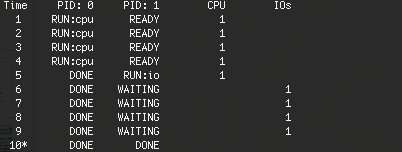
\includegraphics[width=\linewidth]{images/worksheet_1_solution_1.png}
    \end{center}

    \item

    Yes. Switching the order does matter.

    \bigskip

    When the order is switched, the process 2 with I/O runs, and the process 2 enters
    the blocked state.

    \bigskip

    While at blocked state, the other process executes.

    \bigskip

    Since both take 4 seconds, by the time process 2 finishes, process 1 is finished.

    \bigskip

    Thus, total of 6 seconds are taken.


\end{enumerate}

\end{document}